%!TEX root = ../Thesis.tex
\chapter{Experimental results}
\label{sec:results}

%--------------------------------------------------------------------------------
\clearpage
\section{Initial investigation: WAFFLE experiment}
\label{sec:waffle}

Placeholder

The data set and campaign metadata have been published on DTU's data repository (\cite{waffle_dataset}).

%--------------------------------------------------------------------------------
\clearpage
\section{Addendum: Key results and lessons learned}
\label{sec:waffle_addendum}

Placeholder

%--------------------------------------------------------------------------------
\clearpage
\section{Introduction to second study: 
{\O}sterild Balconies experiment}
\label{sec:balcony_intro}

Building upon the methods and results of the initial investigation, a full scale experiment was planned in conjunction with the New European Wind Atlas (NEWA) project. A primary objective of the campaign was to collect data for the purpose of developing a minute-scale wind forecasting system using upwind observations from the scanning lidars. The resulting {\O}sterild Balconies experiment provides cross-sectional scans of the horizontal wind by performing PPI scans at a height raised above the ground. This avoids the wind shear and height difference problems revealed in the initial investigation.

\noindent
An in-depth report of the research output is presented in the open access journal article Section \ref{sec:balcony_paper} and the Addendum \ref{sec:balcony_addendum1}.

\noindent
The data set and campaign metadata have been published on DTU's data repository (\cite{balcony_dataset}).

%--------------------------------------------------------------------------------
\clearpage
\section{Minute-Scale Wind Speed Forecasting Using Scanning Lidar Inflow Measurements}
\label{sec:balcony_paper}

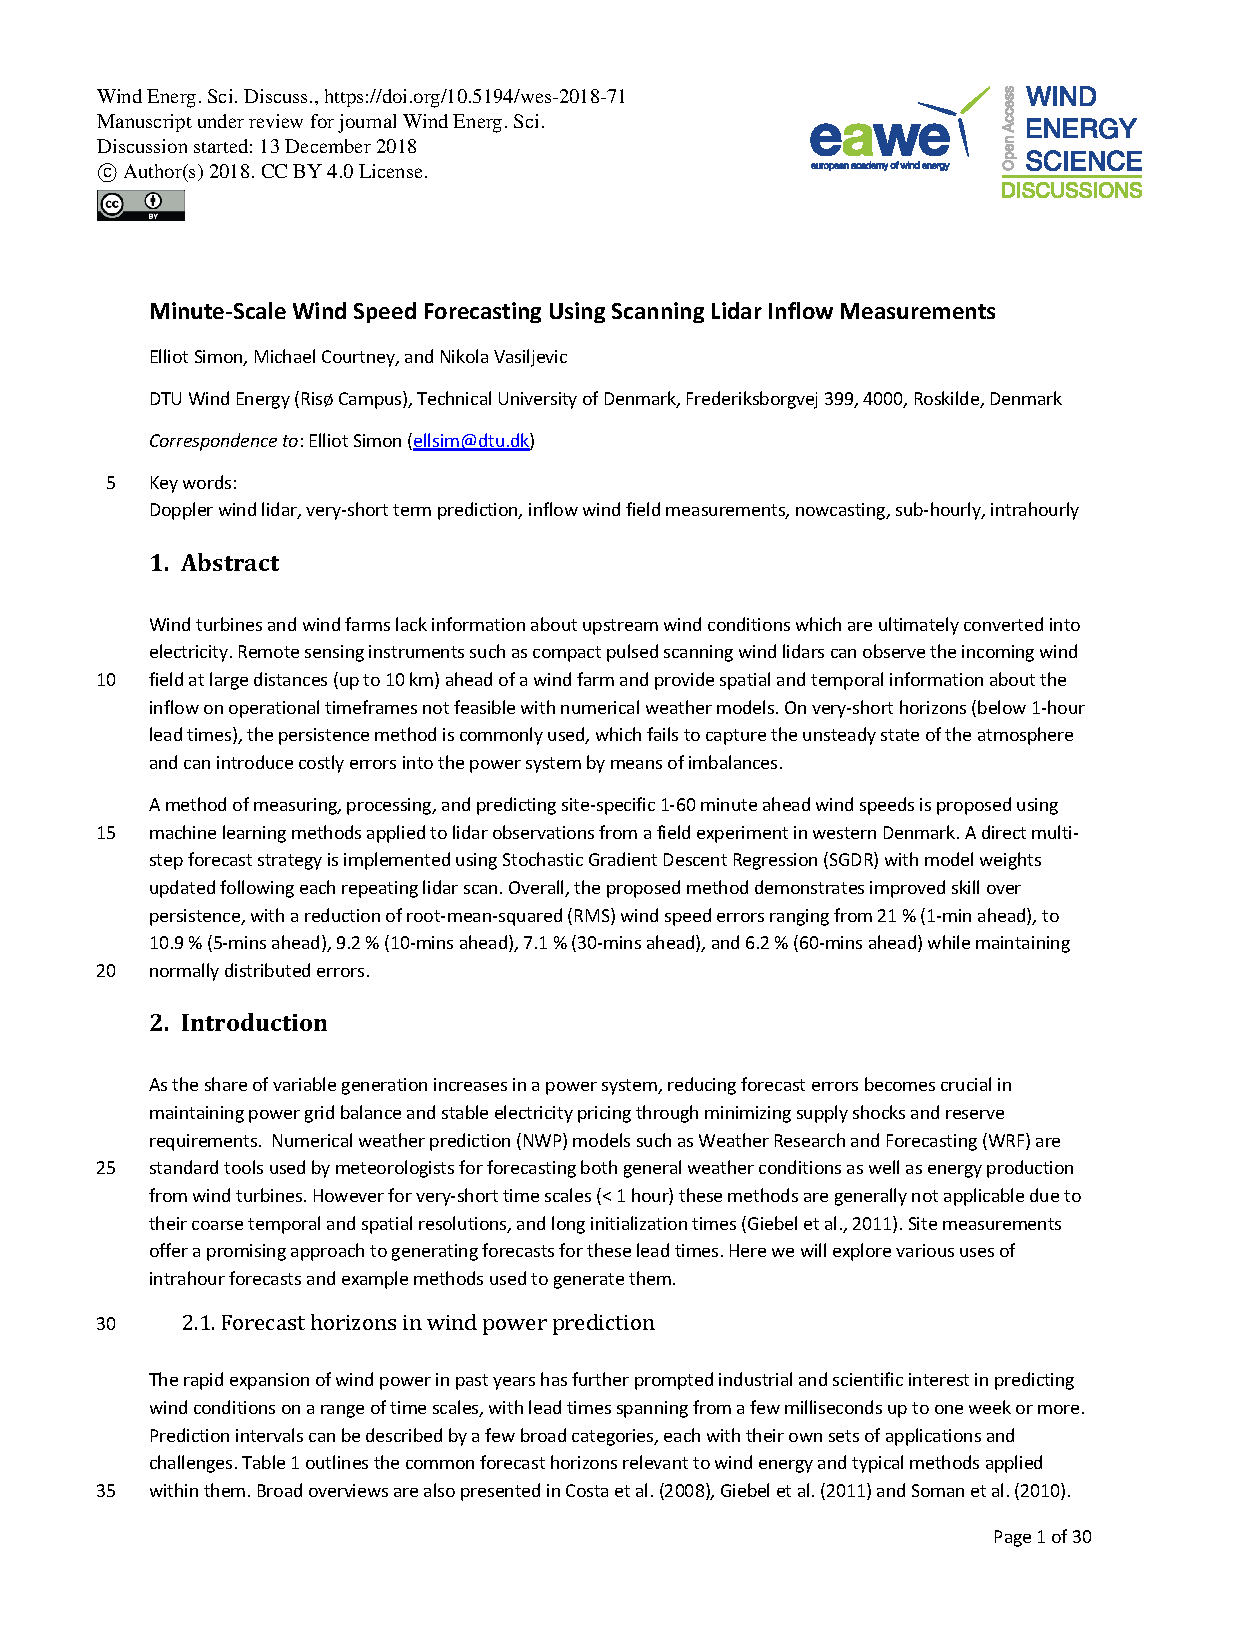
\includepdf[pages=-]{papers/Balcony_paper_WESD.pdf}

%--------------------------------------------------------------------------------
\clearpage
\section{Addendum 1: Weather front event}
\label{sec:balcony_addendum1}

This section expands upon an oral presentation titled "Lidars Lifted: The {\O}sterild Balconies Experiment" given at the 97th American Meteorological Society (AMS) conference in Seattle (\cite{simon_lidars_lifted_2017}).

During the first phase of the Balconies experiment while the scanning lidars were deployed at 50 m above ground level (AGL),
a weather event was encountered with a potentially high impact for an operational wind turbine or wind farm.

At approximately 6PM UTC on the 6th of June 2016, the arrival of a cold front drastically changed the wind regime at the test site. Although it did not cause a significant wind speed ramp, the wind directions of the two air masses were diametrically opposed. The result was a near instant 180 degree shift in wind direction (from 130 to 310 degrees) as the frontal advection displaced the formerly presiding conditions. 

This example of sudden and extreme veer has undesired and potentially damaging effects for a wind turbine. From an energy production perspective by requiring significant time and control adjustments to adapt to the new conditions, and from a loads perspective by introducing a sudden and extreme loading of the rotor and tower structure which is outside of normal operating conditions.

Figure \ref{fig:balcony-front-mast} presents a meteorological look into the event using measurements from the northern aircraft warning tower at {\O}sterild.

\begin{figure}[htbp]
    \centering
        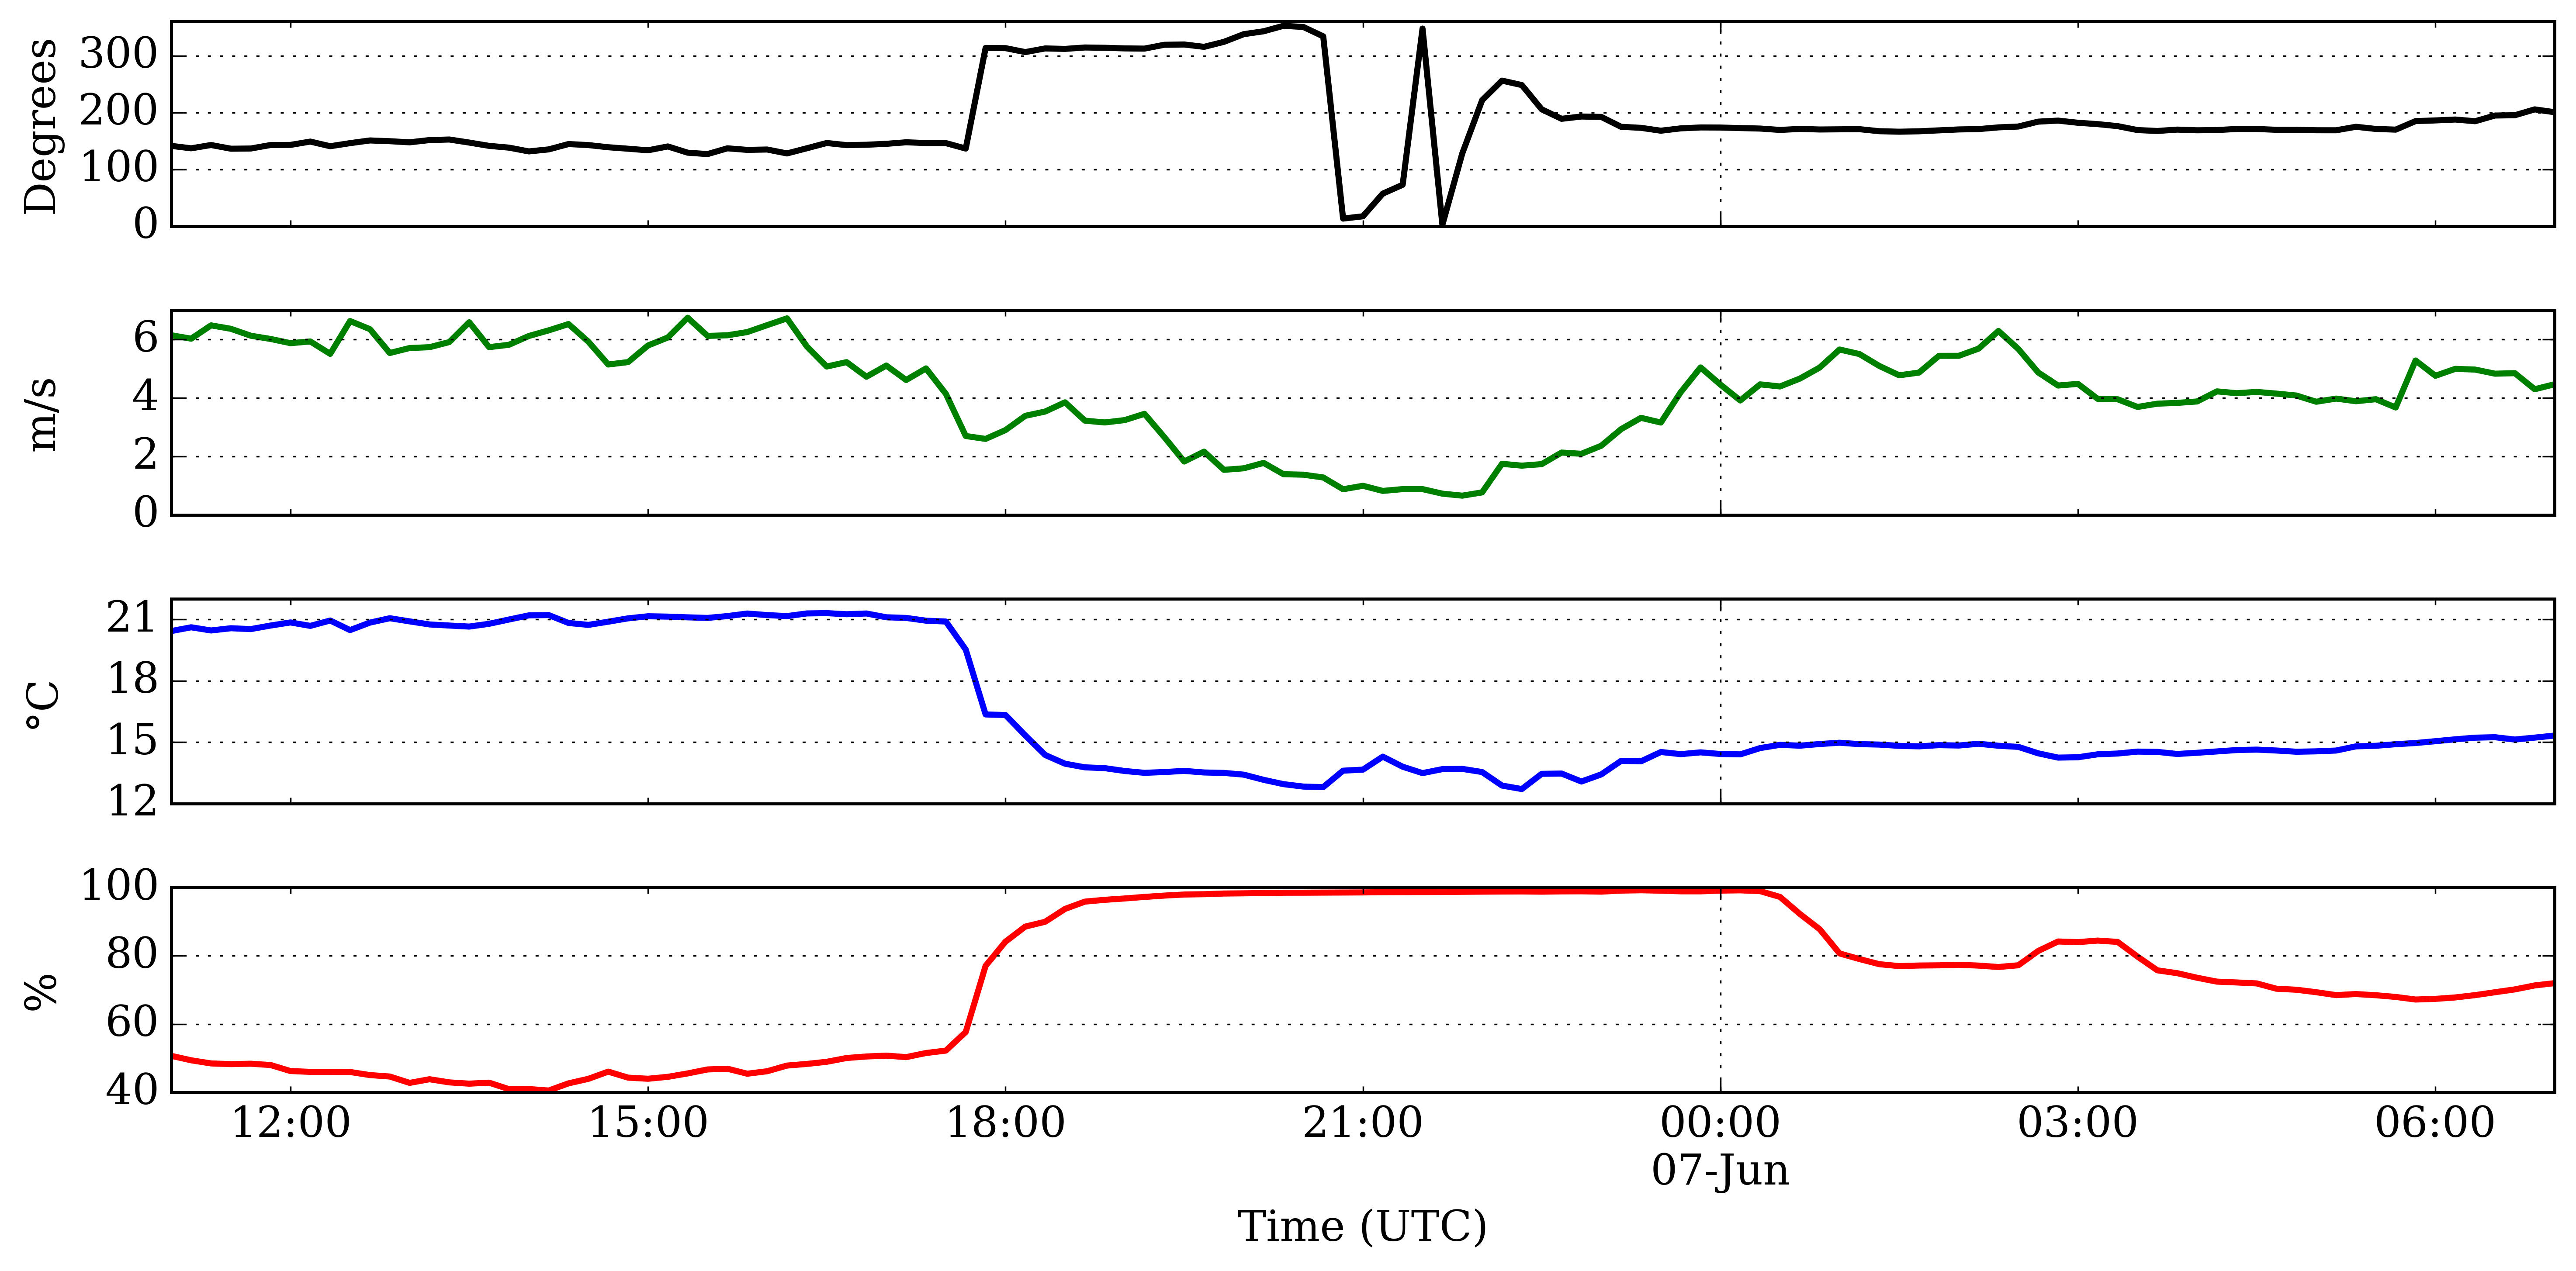
\includegraphics[width=1.0\textwidth]{graphics/results/balcony-addendum/balcony_front_mast.png}
    \caption{Mast measurements during a passing cold front at {\O}sterild test center on June 6-7, 2016.
    Top panel: Wind direction at 40 m AGL. Second panel: Wind speed at 40 m AGL. Third panel: Temperature at 37 m AGL. Bottom panel: Relative humidity at 7 m AGL}
    \label{fig:balcony-front-mast}
\end{figure}

The event is clearly visible in the lidar observations from the Sirocco unit, shown in Figure \ref{fig:lidar_front_ppis_8up}. The frontal boundary is located where the sign of the radial speeds switch from positive (outflow) to negative (inflow). It is first detected 7 km away from the mast position, and the propagation can be tracked over a 2-hour period as it approaches the test site.

% need to clear page before & after this figure as it's huge!
\clearpage
\begin{figure}[htbp]
    \centering
        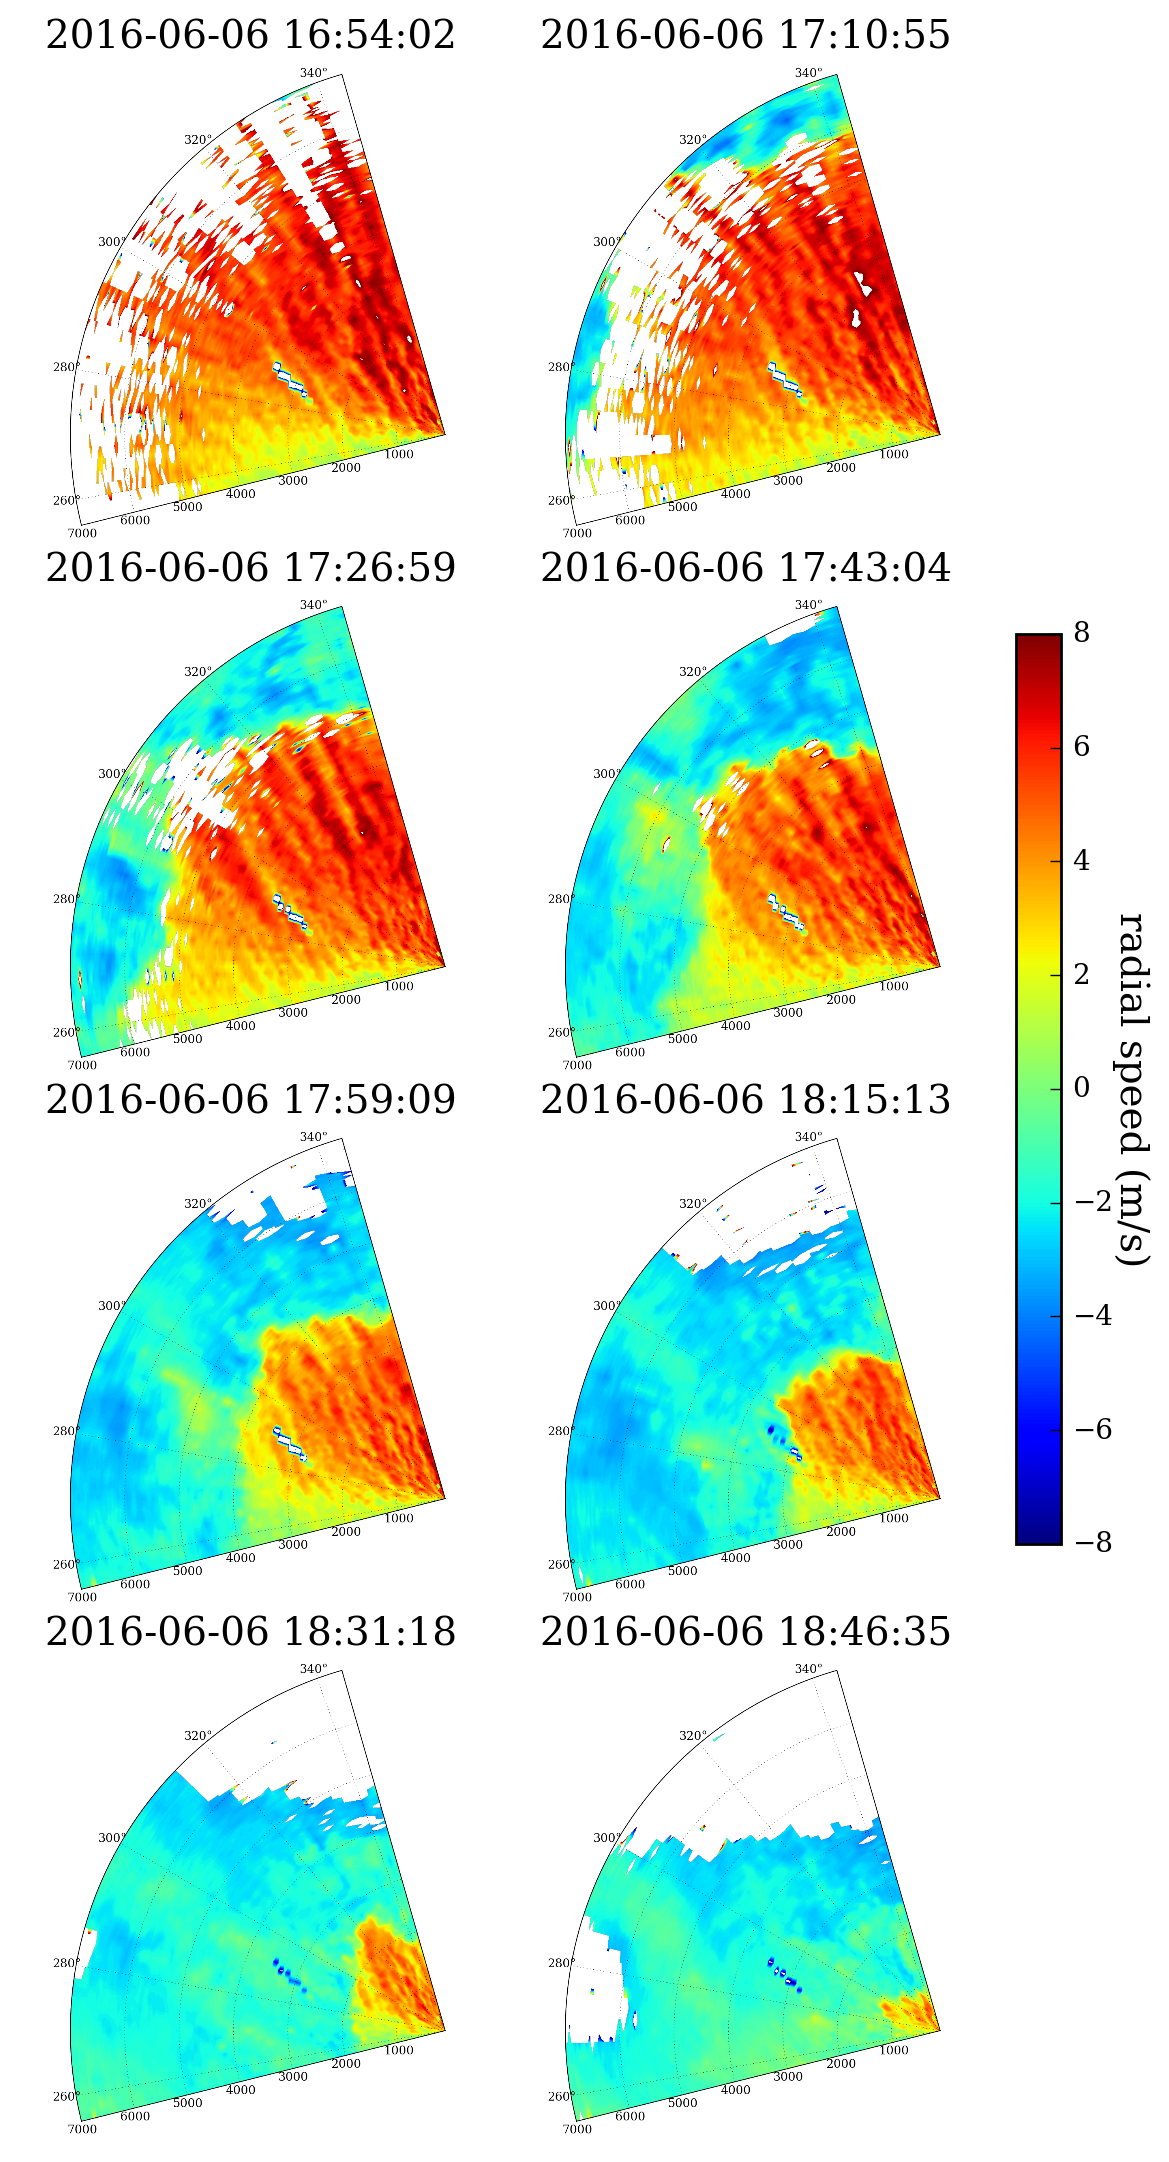
\includegraphics[width=1.0\textwidth, height=1.0\textheight, keepaspectratio]{graphics/results/balcony-addendum/lidar_front_ppis_8up.png}
    \caption{Lidar observations of the frontal passage event from the Sirocco unit. Images are single PPI scans spaced 15-minutes apart. Timestamps are in UTC format}
    \label{fig:lidar_front_ppis_8up}
\end{figure}
\clearpage

This event is an example of a very difficult to forecast phenomenon. Statistical methods including persistence and autoregressive (AR) models will fail spectacularly as there is no connection between the recent past and impending conditions. While physical approaches including numerical weather prediction (NWP) models are in many cases able to predict the existence of a passing weather front, correctly predicting the precise timing is notoriously difficult (phase error).

To further examine the usefulness of the upwind lidar system in capturing the event, predictions from an NWP model were compared with the local site measurements. 
Weather Research and Forecasting (WRF) version 3.5.1 model outputs at 2 km spatial resolution and 1 hour temporal resolution were obtained from Andrea Hahmann at DTU Wind Energy. The domain is shown in Figure \ref{fig:wrf_grid_annotated} along with the grid cell nearest to the met-mast. The distance from the met-mast position to the nearest grid cell is 1.16 km.

\begin{figure}[htbp]
    \centering
        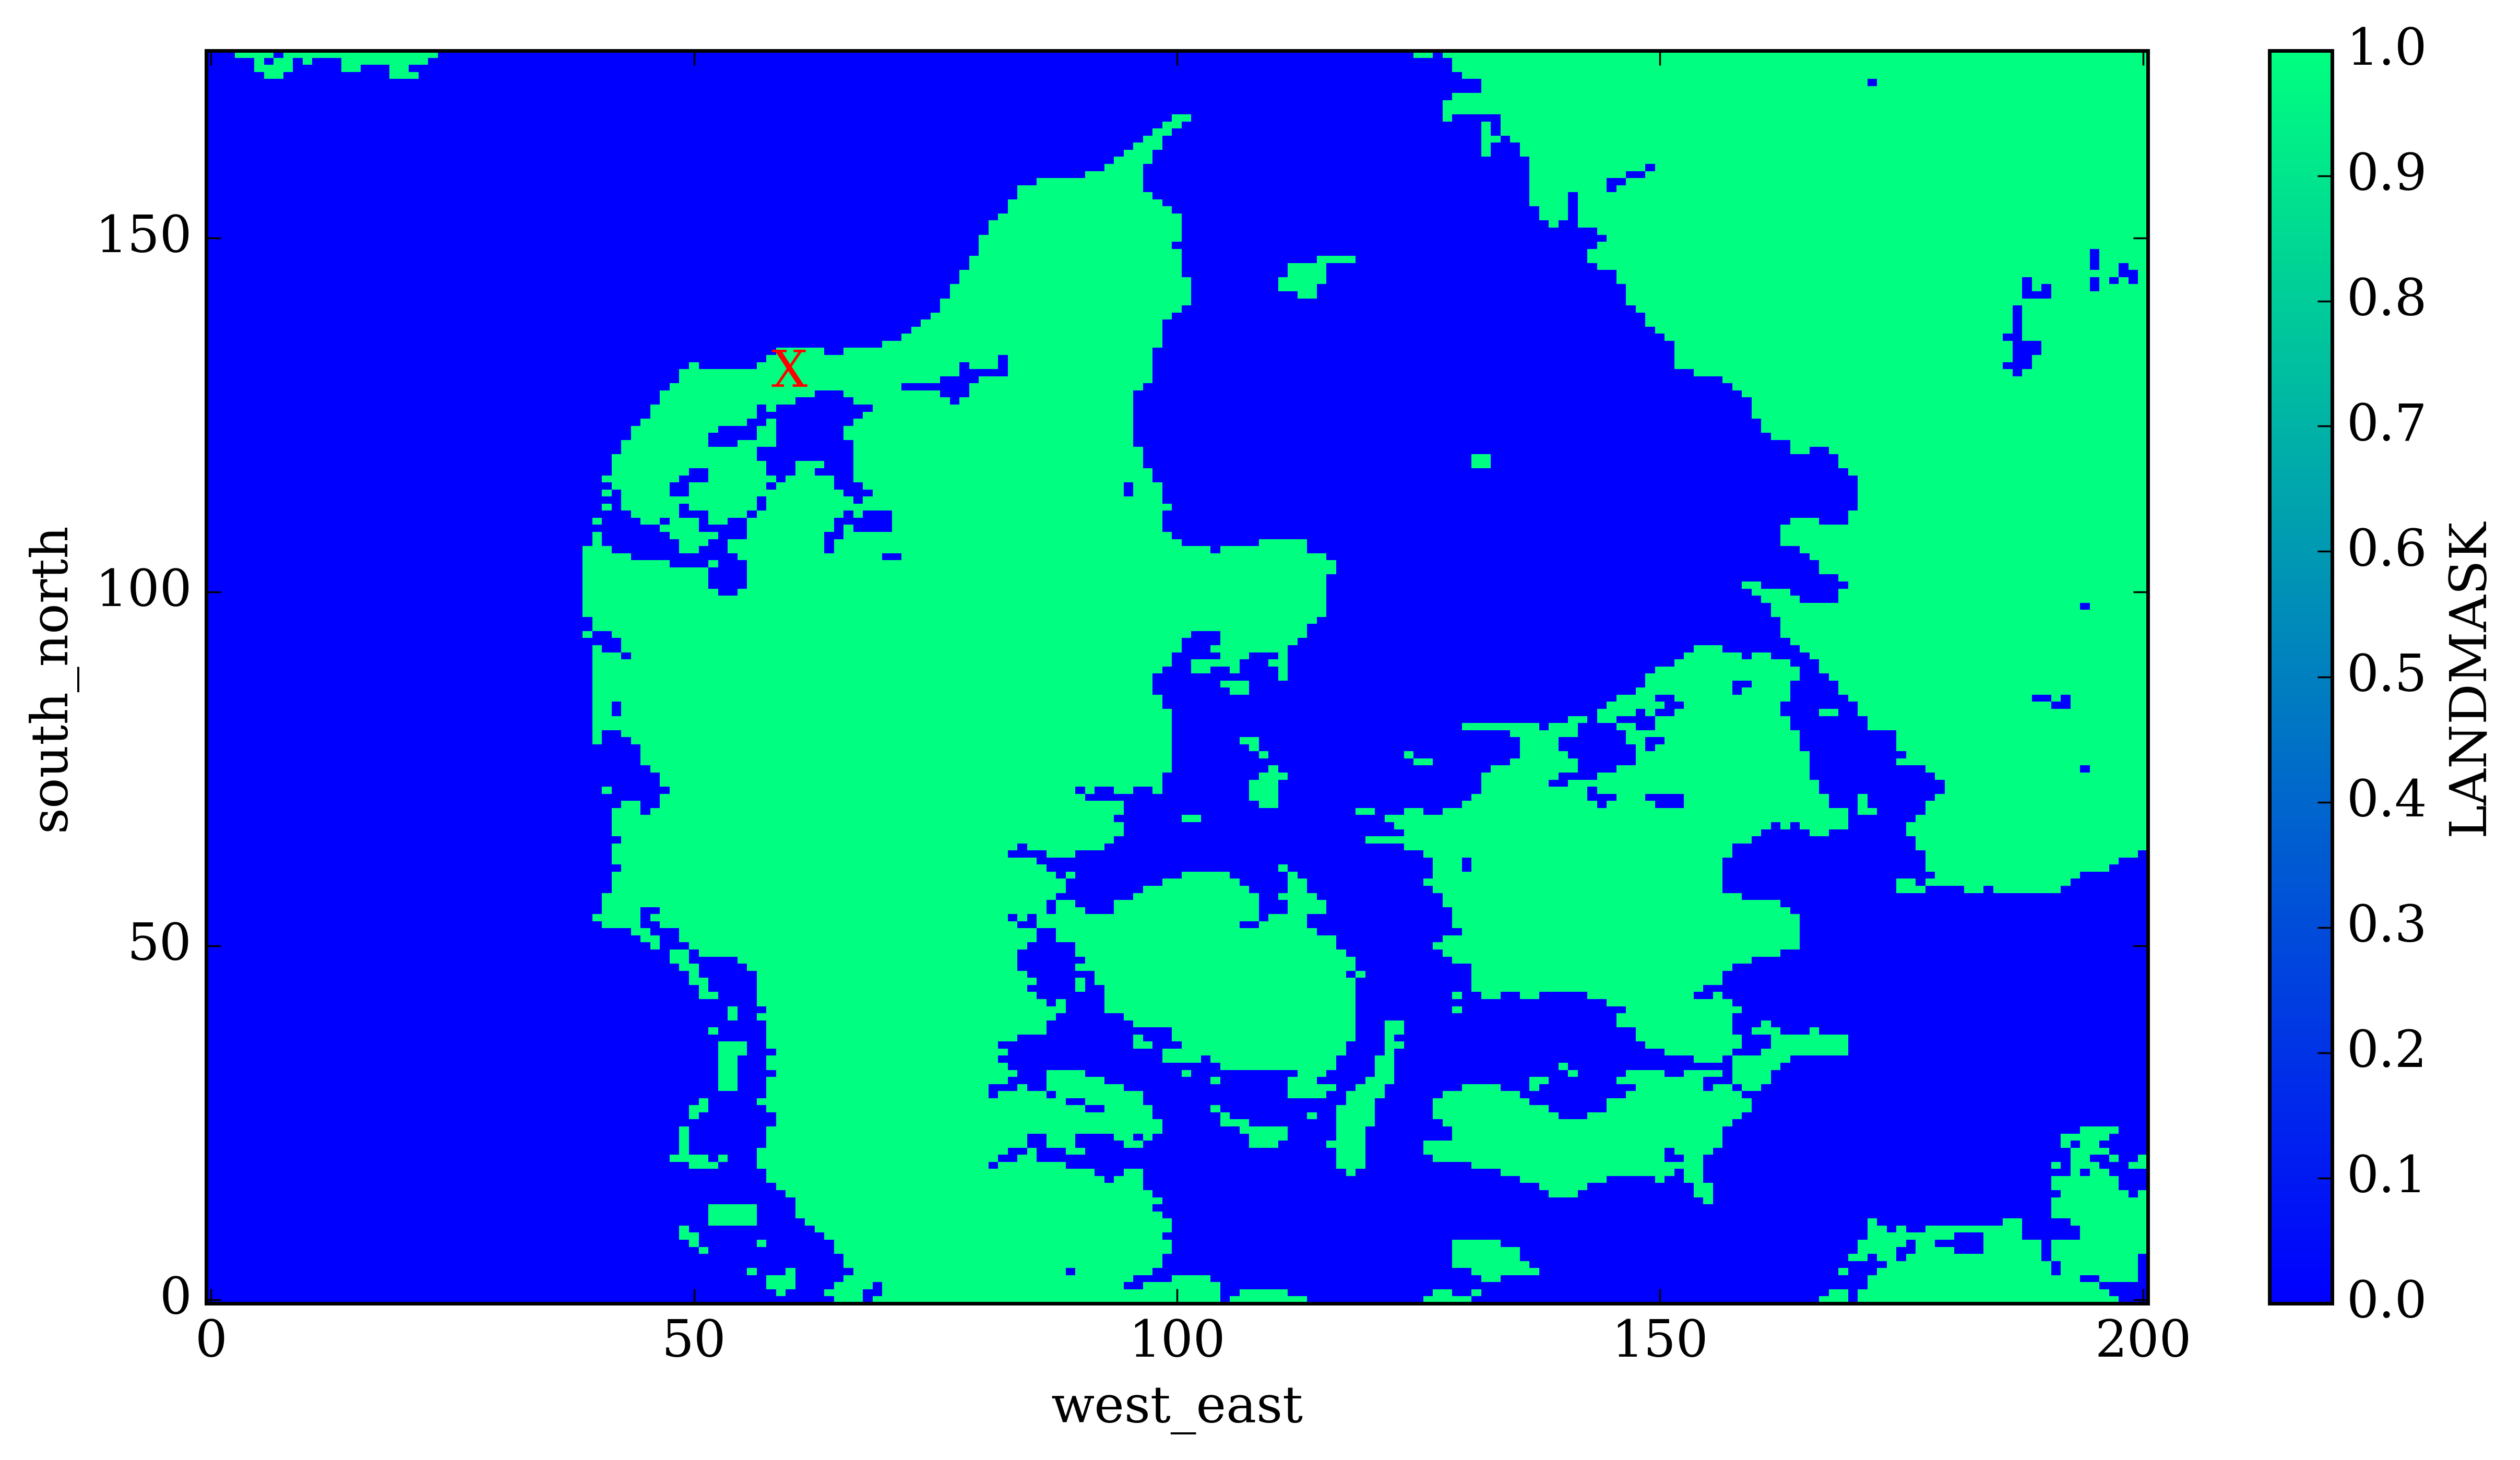
\includegraphics[width=0.75\textwidth]{graphics/results/balcony-addendum/wrf_grid_annotated.png}
    \caption{Domain for WRF simulation, with a red X denoting the chosen grid cell nearest to the met-mast}
    \label{fig:wrf_grid_annotated}
\end{figure}

Four runs: two initialized on June 5th at 0Z (midnight UTC) and 12Z (noon UTC), and two initialized on June 6th (0Z and 12Z) were used to make comparisons between wind speed and direction predictions and the reference site measurements. The met-mast measurements have been converted to UTC time for synchronization with the WRF model outputs.

\begin{figure}[H]
    \centering
        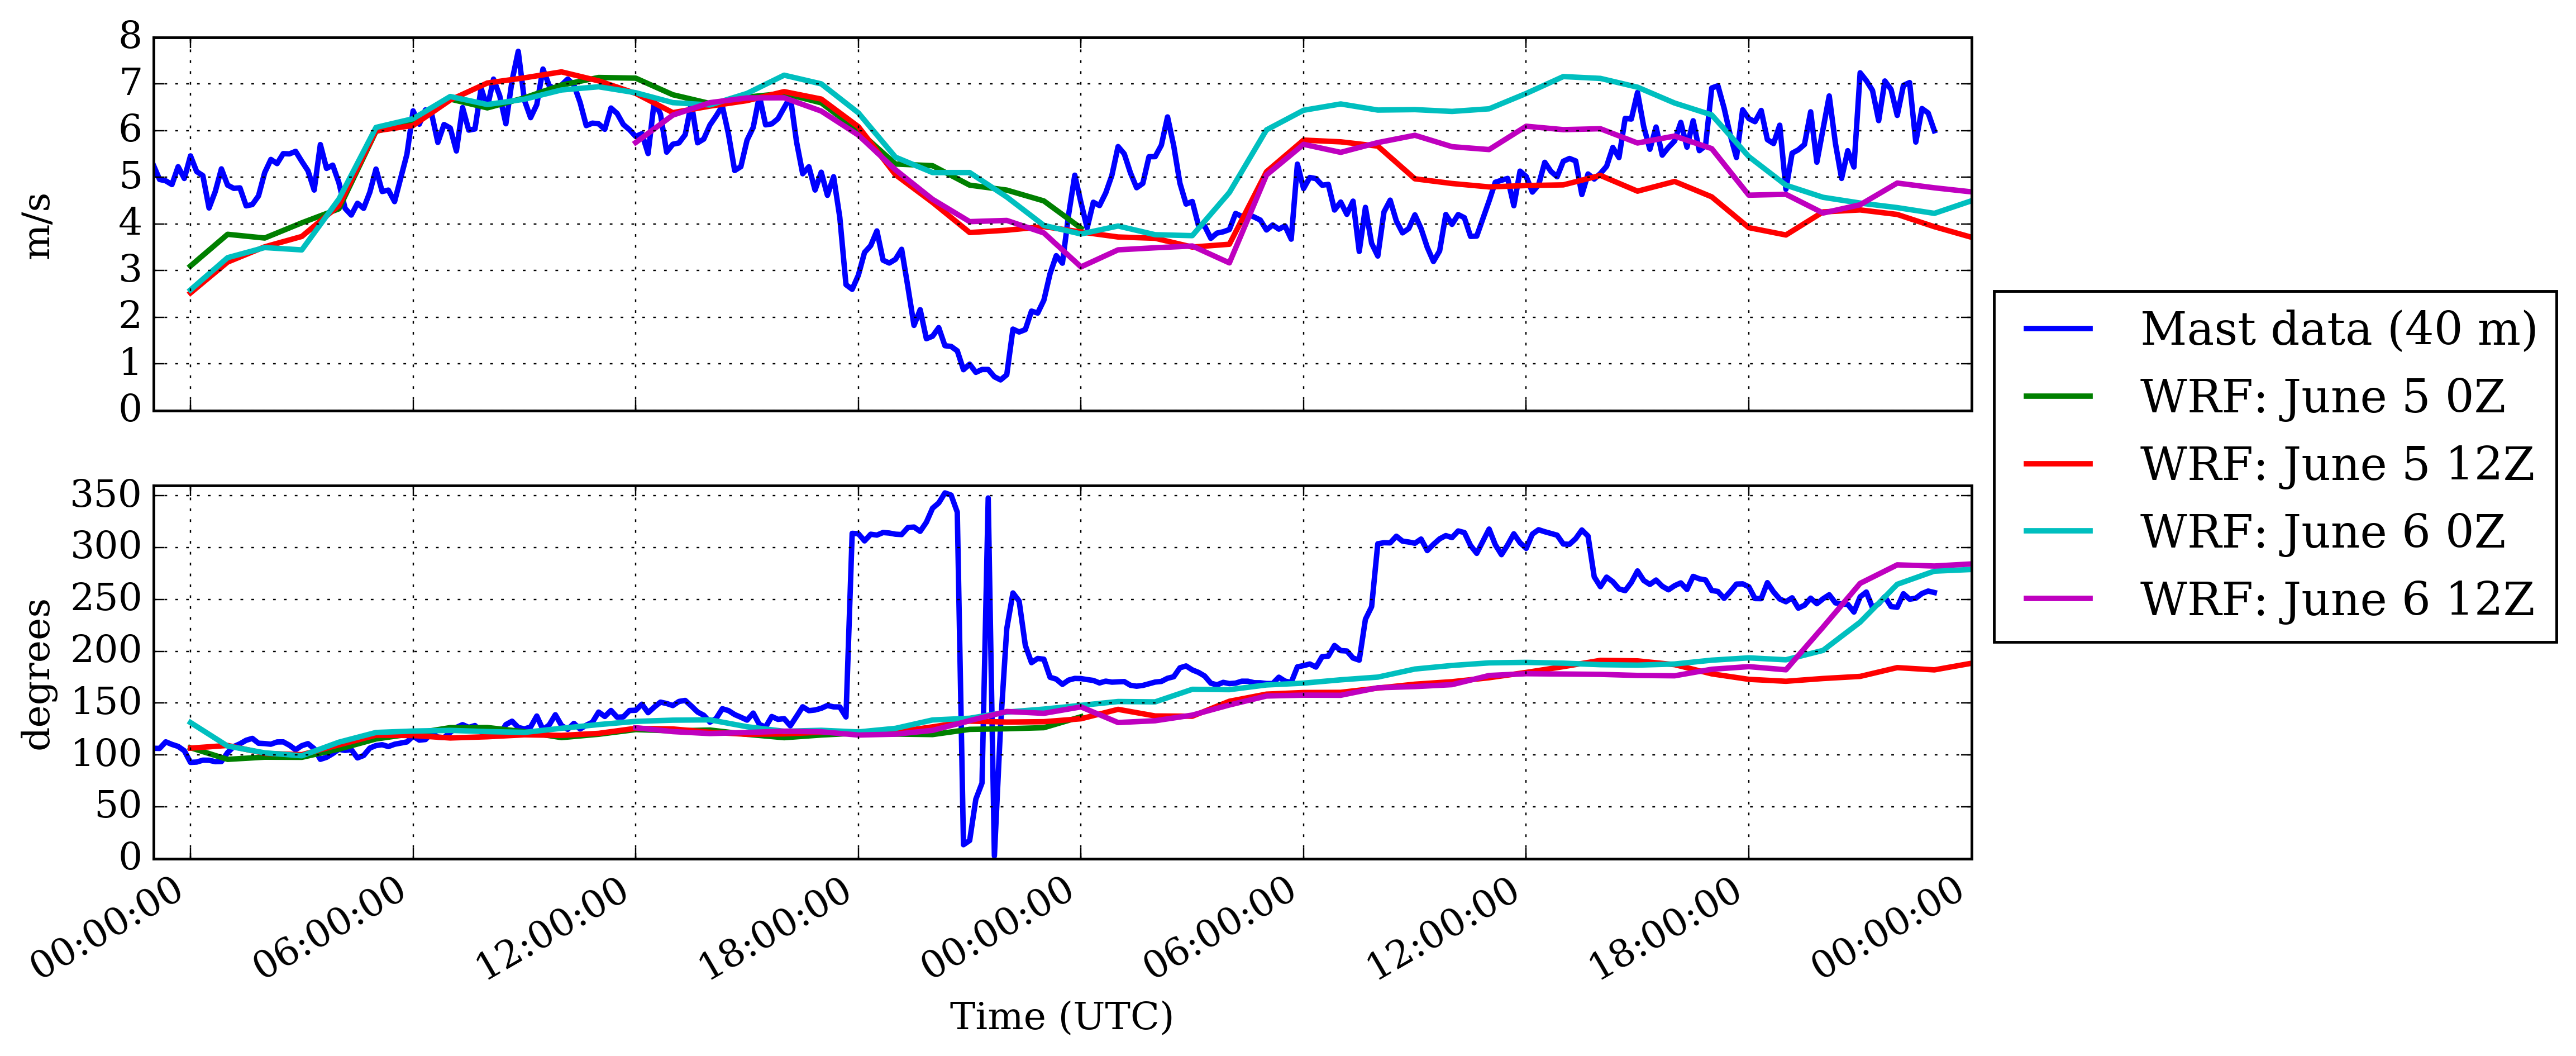
\includegraphics[width=1.0\textwidth]{graphics/results/balcony-addendum/wrf_mast_comparison.png}
    \caption{Comparison of four WRF model predictions with reference met-mast measurements}
    \label{fig:wrf_mast_comparison}
\end{figure}

WRF results are largely consistent across the four runs. Predictions between midnight and 6 PM UTC appropriately match the observational data from the met-mast. However, after this time the forecast does not capture the direction change which is a result of the event observed by the lidar. A further example of a timing (phase) error can be seen in the second direction veer occurring at 8 AM but forecasted to occur 12 hours later.

In summary, the lidar observations have demonstrated a clear value in capturing and tracking a weather event of potential concern as it approaches a wind turbine or wind farm. The event was not predicted by the WRF NWP approach, but was detected 2 hours beforehand by the scanning lidar and its propagation was tracked until arriving to the met-mast position.

This result supports the use of upwind lidar data for detecting and forecasting the arrival of large scale events at a local site. Particularly for sites with recurring localized weather patterns, this application carries promise when used as a classification and warning system to the operator or automated control systems.

%--------------------------------------------------------------------------------
\clearpage
\section{Addendum 2: Key results and lessons learned}
\label{sec:balcony_addendum2}

\begin{itemize}
    \item I did something good
    \item I did something else good
    \item And maybe possibly a third good thing?
\end{itemize}

%--------------------------------------------------------------------------------
\clearpage
\section{Introduction to third study: LASCAR experiment}
\label{sec:lascar_intro}

Placeholder

The data set and campaign metadata have been published on DTU's data repository (\cite{lascar_dataset}).

%--------------------------------------------------------------------------------
\clearpage
\section{Minute-Scale Wind Vector Forecasting Using Scanning Lidar Inputs to a Convolutional LSTM Neural Network}
\label{sec:lascar_paper}

Placeholder for LASCAR paper
%\includepdf[pages=-]{papers/LASCAR_paper.pdf}

%--------------------------------------------------------------------------------
\clearpage
\section{Addendum: Key results and lessons learned}
\label{sec:lascar_addendum}

Placeholder